\chapter{Program flowchart}\label{app:flowchart}

A flowchart is a conceptual aid which highlights input and output that a program should have, as well as the consequences of any decisions that it must make. Sometimes, these will include \textit{pseudocode}, which mimics some of the more common coding structures in a universal way. (For instance, you might say `loop over all array addresses'.)\\

This particular flowchart indicates a program that reads three numbers from the terminal, and then produces the largest of the numbers back to the terminal. The colour scheme is not mandatory, but helps the reader to know what is going on at a glance.\\

This flowchart was drawn with the free `Lucidcharts' extension to Google Docs, from which the result was exported as an \texttt{svg} file, and any unnecessary features were then cropped out with Inkscape. Choose any method you wish to create your own flowchart!

\begin{figure}[h!]
\begin{center}
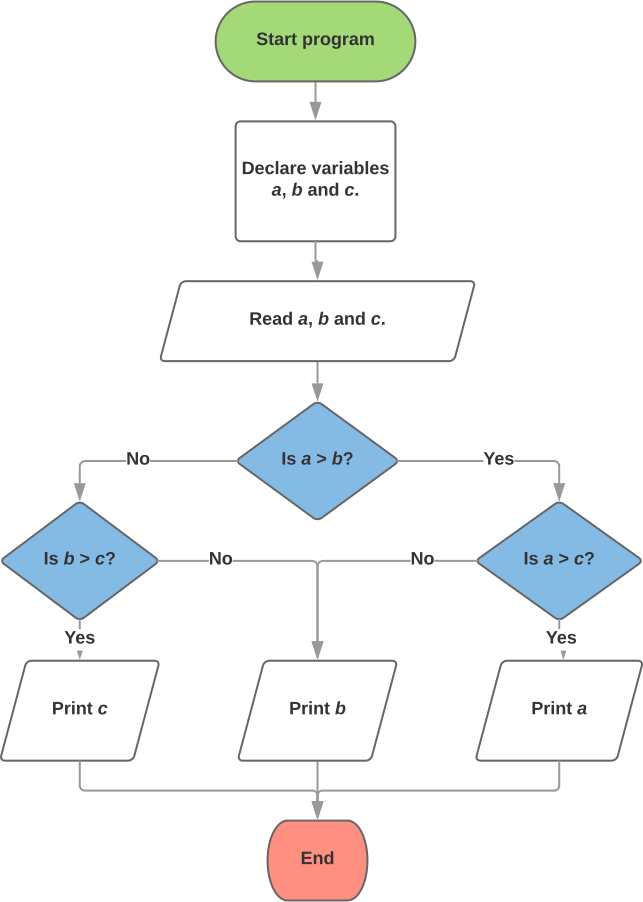
\includegraphics[width=0.50\linewidth]{figures/flowchart.pdf}
\end{center}
\caption{A flowchart for the determination of the largest of three user-selected numbers.}
\label{fig:flowchart}
\end{figure} 